\subsectionaddtolist{توضیح کد}

در ابتدا یک سرور FTP با استفاده از کتابخانه pyftpdlib بالا میاوریم:


	{
	\centering{
	
	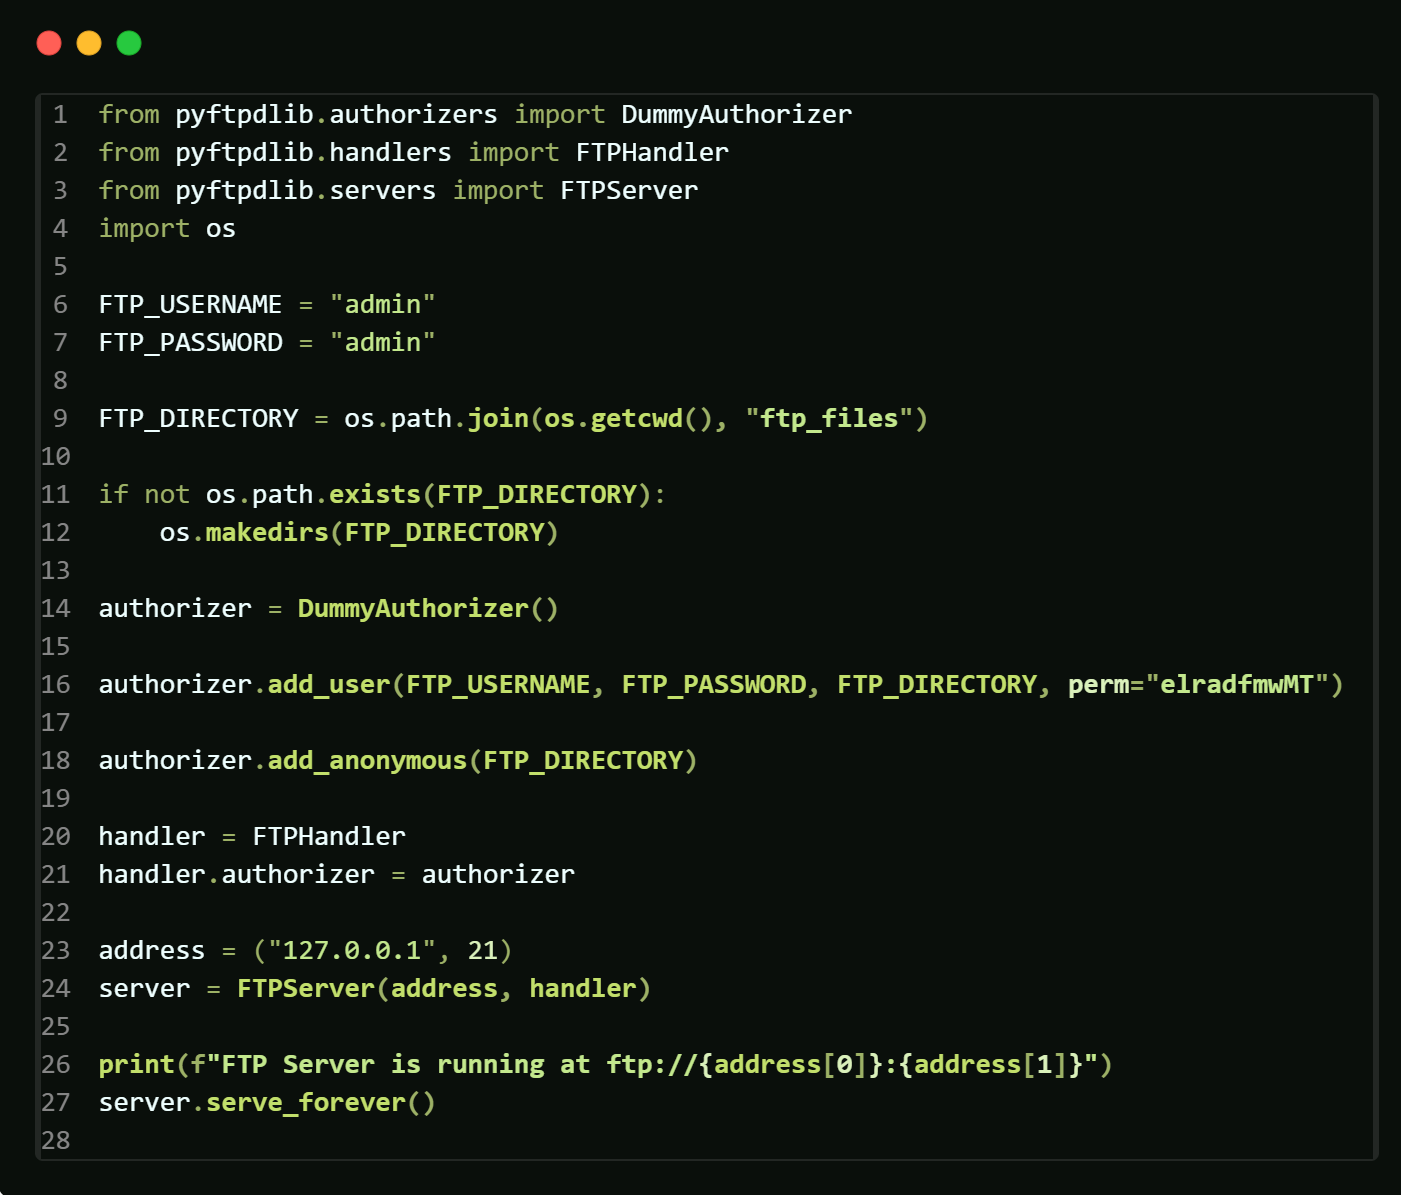
\includegraphics[width=0.5\linewidth]{figs/1}
	
	}
	}

با توجه به اینکه این سرور برای تست است، یوزرنیم و پسورد آن را هاردکد کرده و در کد سرور و کلاینت استفاده میکنیم. سرور FTP ما روی فولدر $ftp\_files$ است و تمامی فایل ها در آن پوشه سرو خواهند شد.


حال به سراغ کد سرور میرویم و مرحله به مرحله آن را شرح میدهیم.
ما از کتابخانه های اصلی و مهم Socket و Threading و ftplib استفاده میکنیم. همچنین یک آبکجت برای Clientهای متصل و یک Counter برای ID آن ها در نظر گرفته ایم. 

{
	\centering{
		
		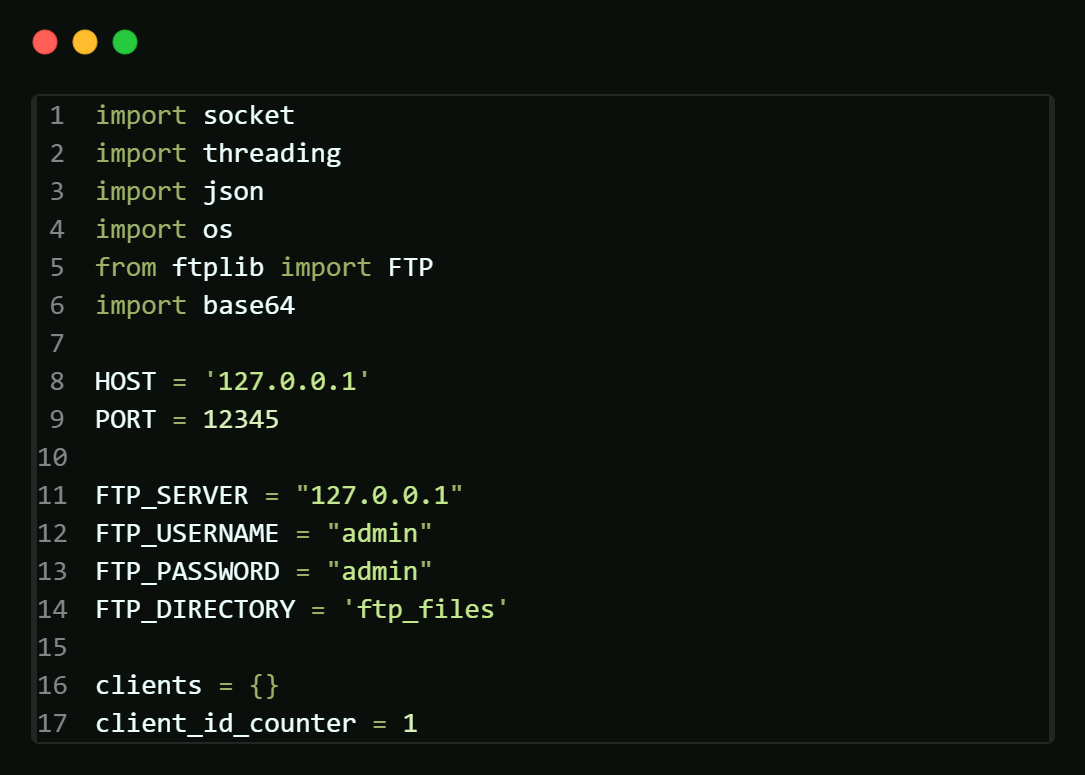
\includegraphics[width=0.5\linewidth]{figs/2}
		
	}
}

\pagebreak

این تابع برای ارسال یک پیغام به Clientهای متصل استفاده میشود. البته میتوان یک کلاینت خاص را استثنا قرار داد و به آن پیغام ارسال نکرد.

{
	\centering{
		
		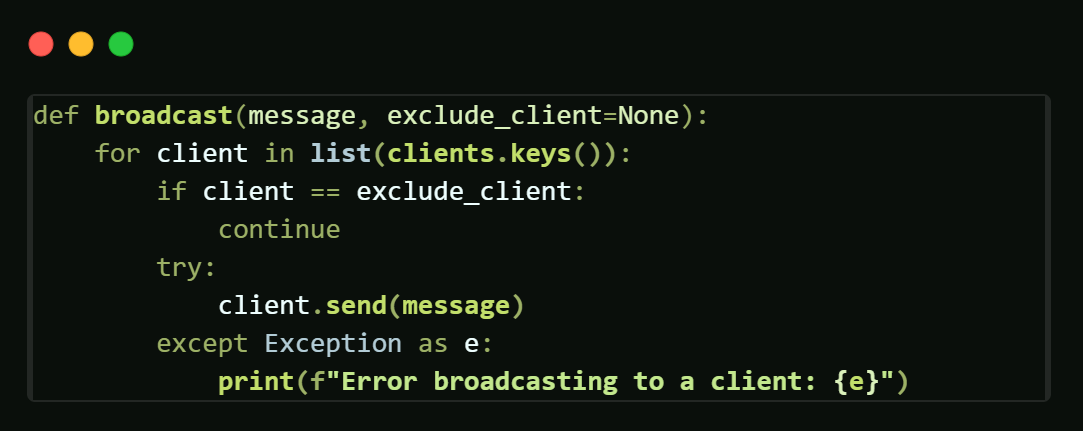
\includegraphics[width=0.5\linewidth]{figs/3}
		
	}
}


یک تابع هم برای نمایش لیست فایل های موجود در سرور FTP استفاده میشود. ابتدا به سرور با استفاده از یوزرنیم و پسورد داده شده وصل میشود و سپس لیست فایل های موجود در فولدر سرو شده توسط FTP را برمیگرداند. اگر به ارور بخوریم یا فایلی وجود نداشته باشد، یک لیست خالی برگردانده میشوند.


{
	\centering{
		
		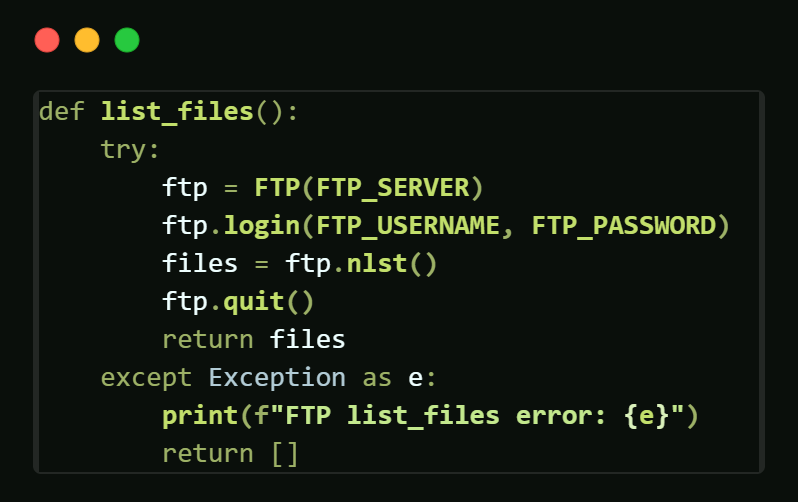
\includegraphics[width=0.5\linewidth]{figs/4}
		
	}
}

این تابع برای دانلود فایل توسط استاد مورد استفاده قرار میگیرد. به این صورت که نام فایل را ورودی میگیرد و سپس فایل را به صورت باینری و در قالب تعدادی بایت برمیگرداند تا بعدا بر روی فایل جدیدی نوشته شود.

{
	\centering{
		
		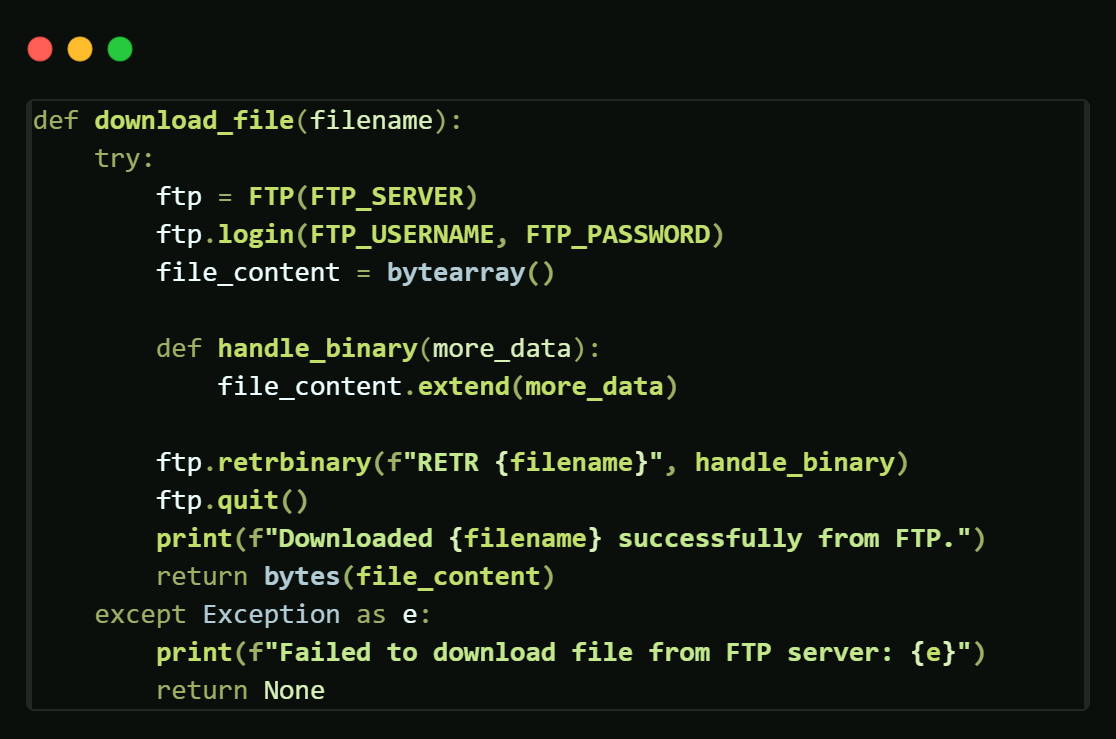
\includegraphics[width=0.5\linewidth]{figs/5}
		
	}
}


\pagebreak


این بخش به نوعی جایگزین رابط گرافیکی برای کاربر سمت سرور است. او میتواند کامندهای زیر 
را استفاده کند و از طریق این تابع، دستور به تابع هندلر اختصاصی آن کامند ارسال میشود.


{
	\centering{
		
		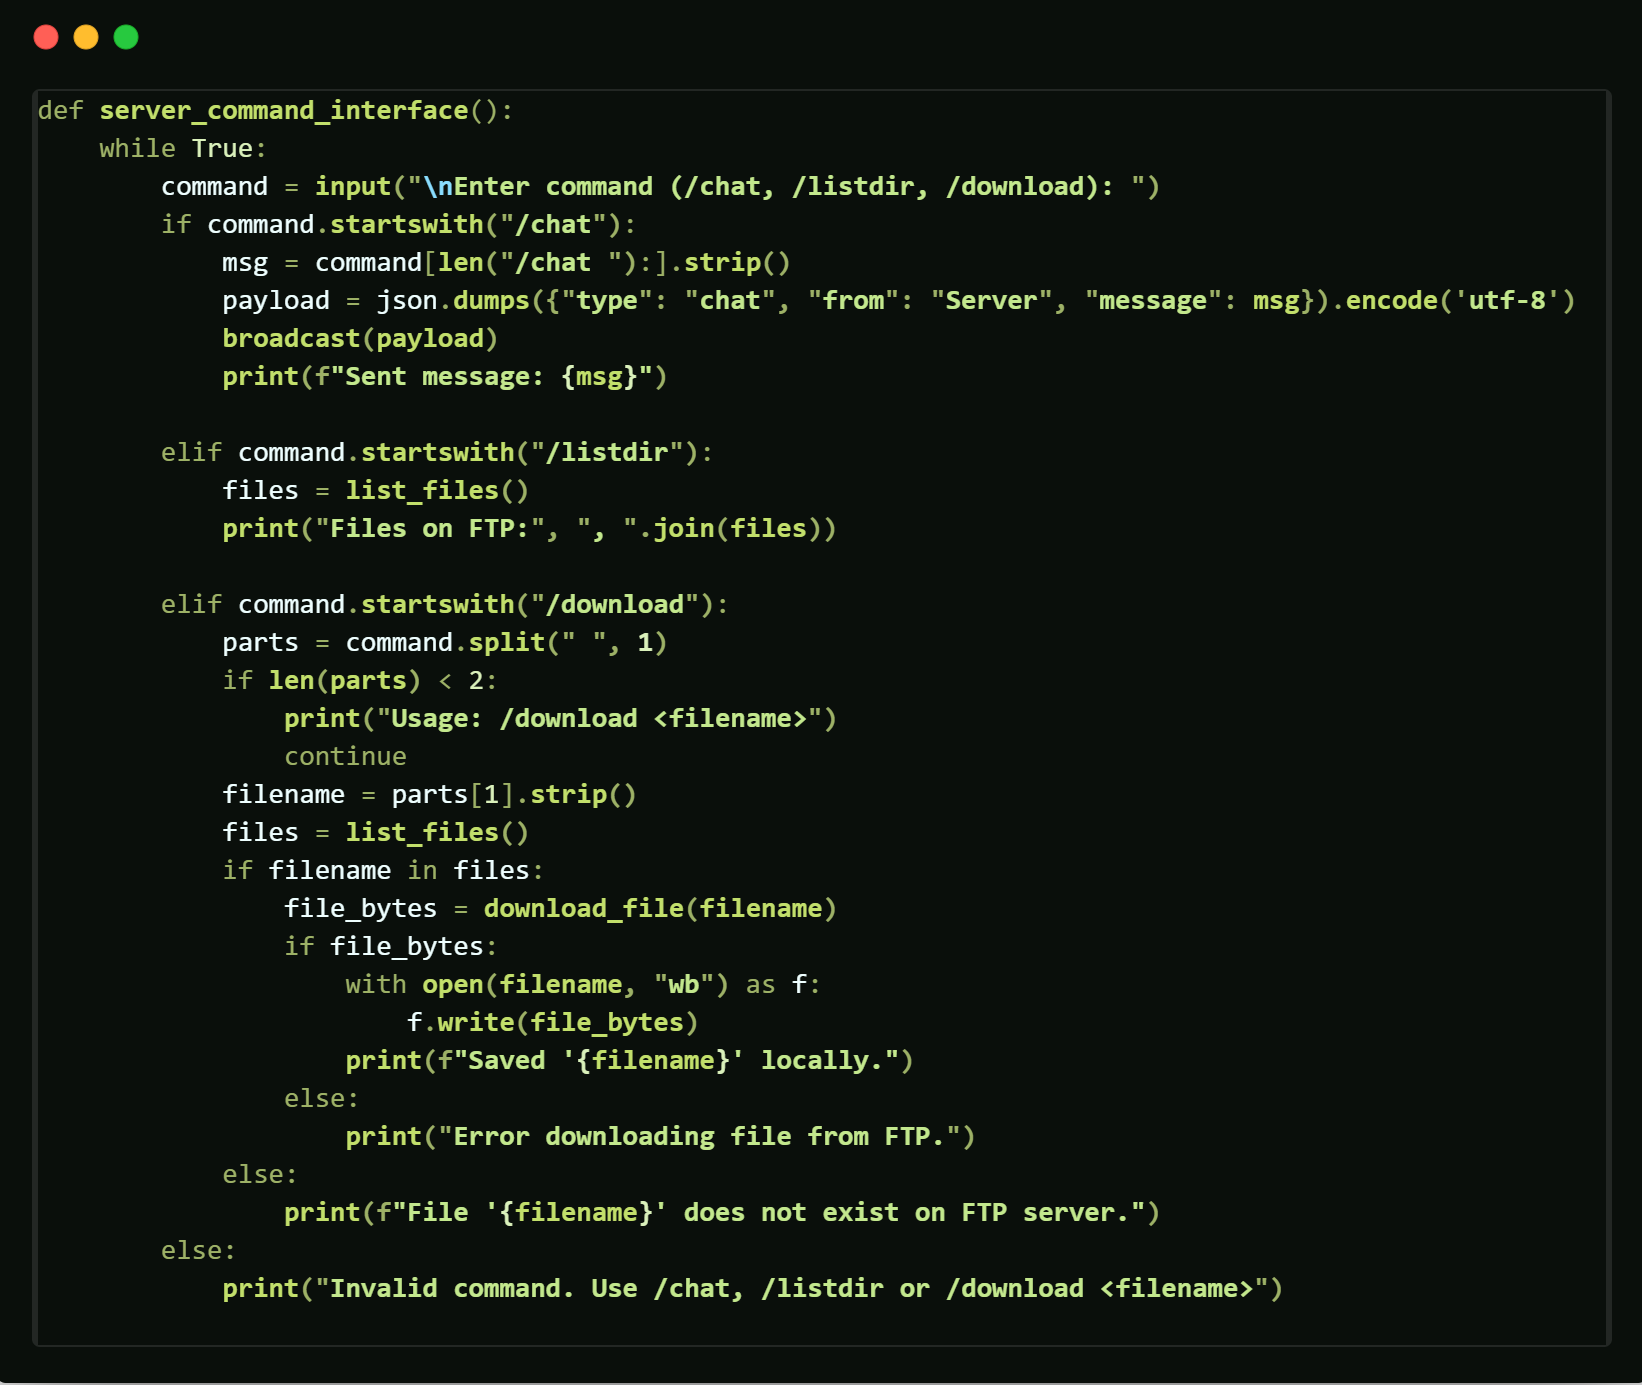
\includegraphics[width=0.7\linewidth]{figs/6}
		
	}
}


در ادامه یک تابع handle\_client هم داریم که به ازای هر Client که به WebSocket ما متصل میشود در یک ترد یک While True ایجاد میکند و دائم منتظر شنیدن دستورات Client است و با توجه به دستور آن، تابع مورد نظر را فراخوانی میکند و پاسخ را در قالب مناسب به آن برمیگرداند. این بخش از کد منطق خاصی ندارد و صرفا زیاده نویسی است. 

بخش اصلی سرور ما این تابع است که سرور را بالا میاورد و به ازای هر کانکشن یک ترد با هندلر مشخص ایجاد میکند.


{
	\centering{
		
		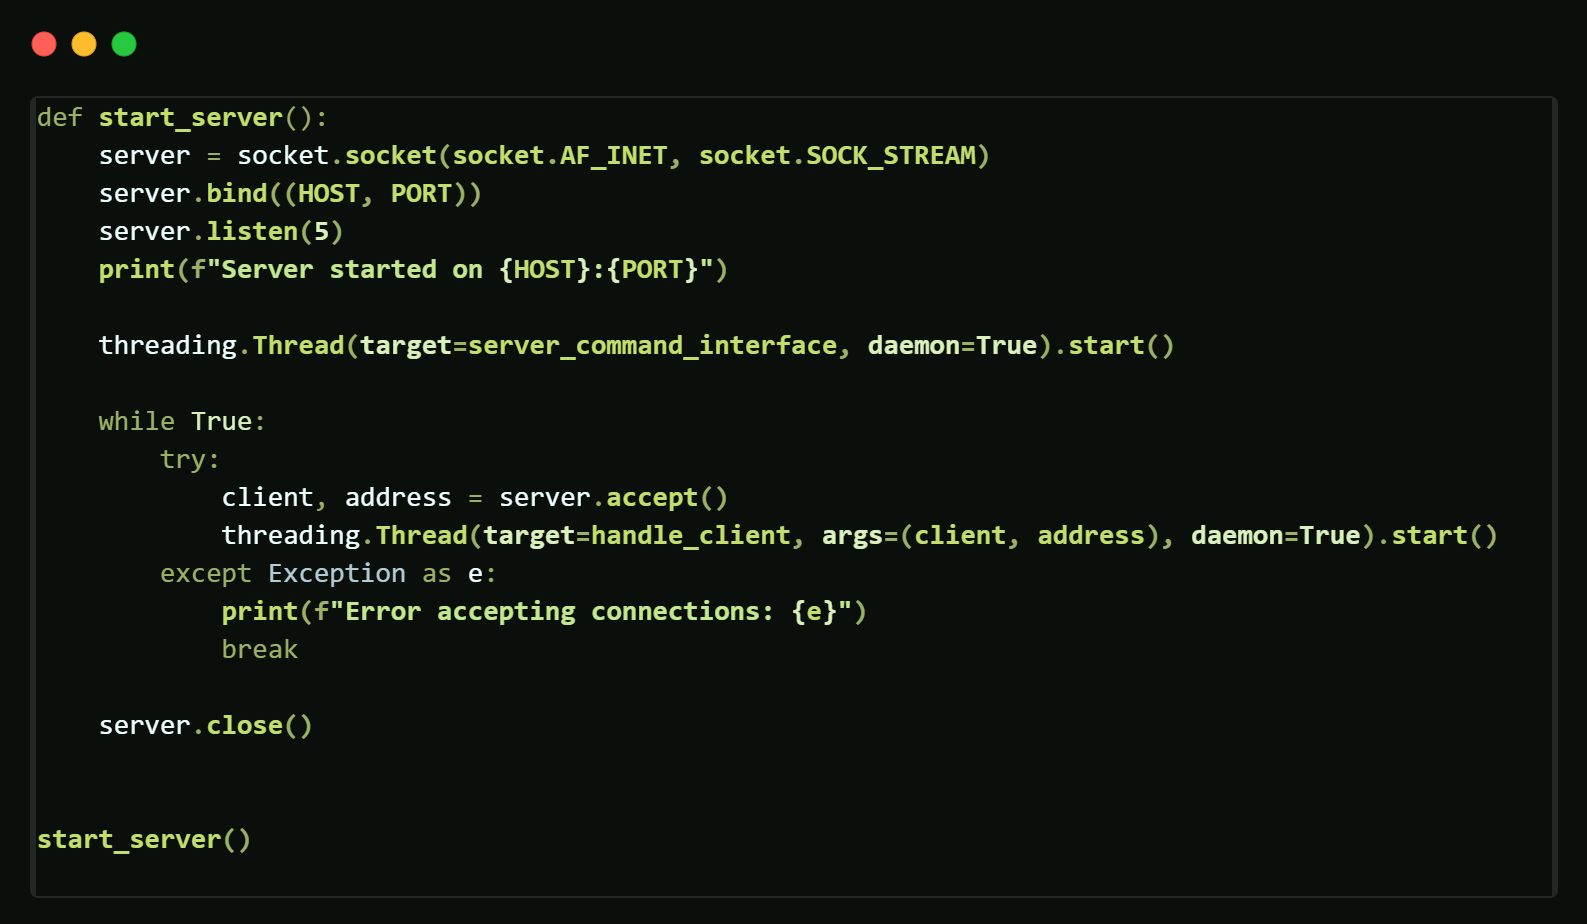
\includegraphics[width=0.7\linewidth]{figs/7}
		
	}
}


حال به سراغ توضیح کدهای Client میرویم. همانند کد سرور، در ابتدا تعدادی کانفیگ اولیه داریم، یک تابع هم برای upload که مشابه کد سرور است و بر روی FTP فایل را اپلود میکند. یک تابع receive\_messages هم داریم که بعد از تشکیل کانکشن، لاجیک خاصی ندارد و صرفا پیام ها را دریافت میکند و در ترمینال برای کلاینت چاپ میکند. 


برای بخش ارسال ایمیل ما از کتابخانه smtplib استفاده کردیم که به smtp server گوگل با استفاده از یوزرنیم و پسورد جیمیل متصل شده و ایمیل را به مقصد مشخص ارسال میکند. بدنه تابع ارسال ایمیل به این صورت است:

{
	\centering{
		
		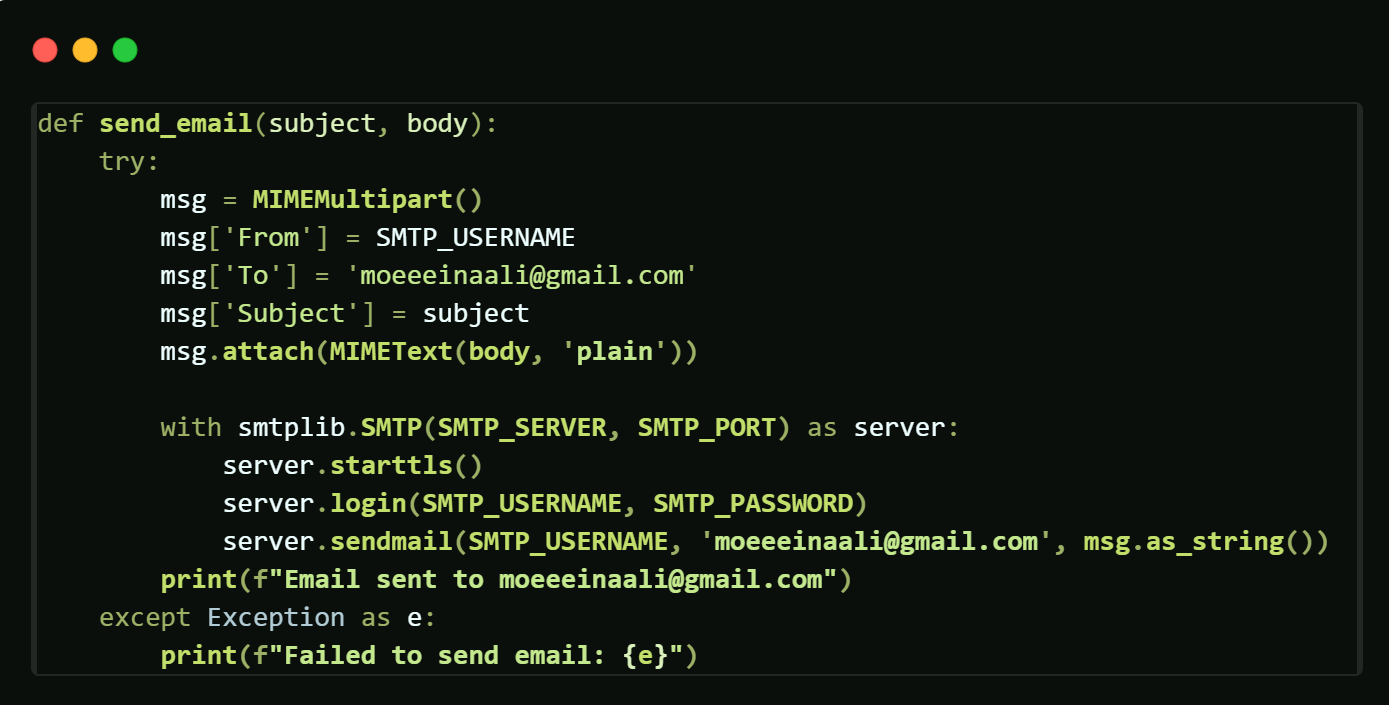
\includegraphics[width=0.7\linewidth]{figs/8}
		
	}
}


بخشی از تابع start\_client به این صورت است، وقتی کد client را ران میکنیم این تابع ران میشود. ابتدا با websocket یک کانکشن با سرور برقرار میکند و سپس در یک ترد جداگانه به پیام های ارسالی از طرف سرور گوش میدهد. (تابع آن را در بخش قبل توضیح دادم) سپس در یک while true نقش واسط کاربر client را اجرا میکند و دستورات کلاینت را دریافت میکند:


{
	\centering{
		
		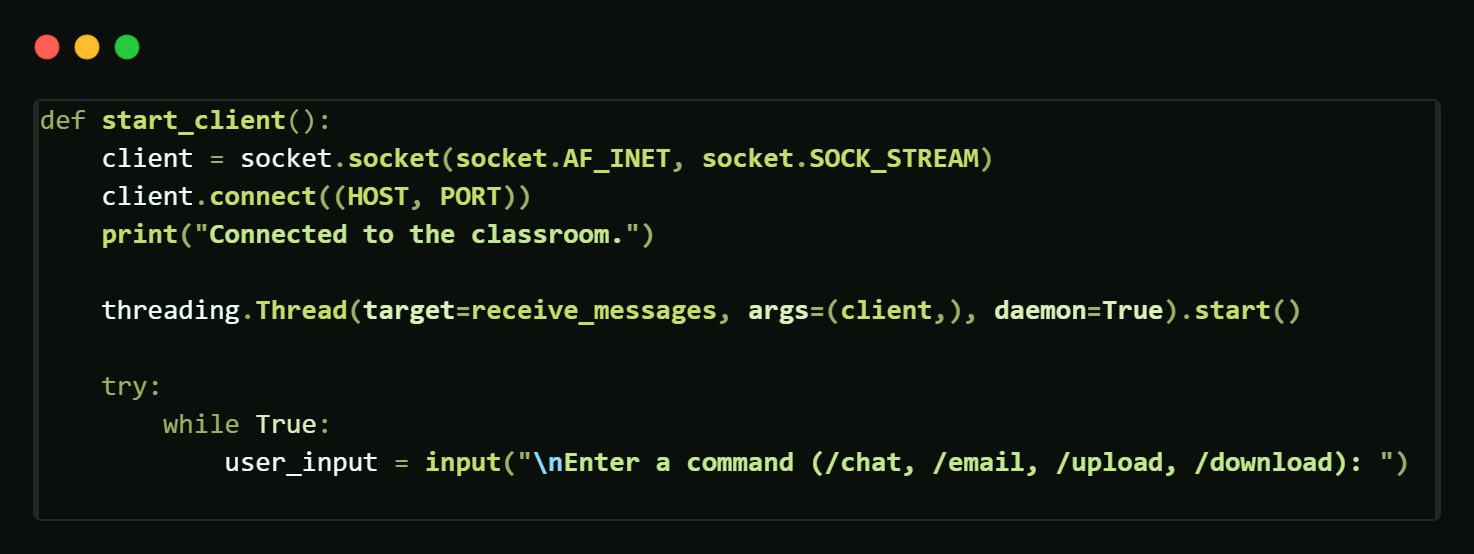
\includegraphics[width=0.7\linewidth]{figs/9}
		
	}
}



\subsectionaddtolist{نتایج اجرای کد}

ابتدا سرور FTP را بالا میاوریم: 

{
	\centering{
		
		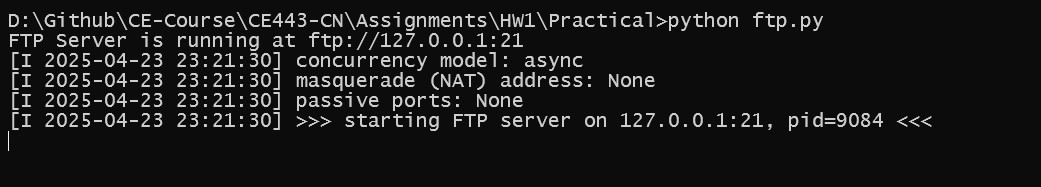
\includegraphics[width=0.7\linewidth]{figs/11}
		
	}
}


سپس سرور استاد را بالا میاوریم: 

{
	\centering{
		
		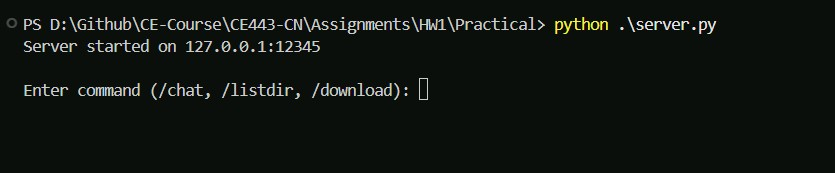
\includegraphics[width=0.7\linewidth]{figs/12}
		
	}
}

\pagebreak

حال با 3 کلاینت مختلف به سرور وصل میشویم. همانطور که میبینید در ابتدای ورود به هر کاربر Welcome Message ارسال شده و آیدی آن را اعلام میکنیم. همچنین به کاربرانی که از قبل  وصل هستند اطلاع میدهیم که یک کاربر جدید اضافه شده است.

{
	\centering{
		
		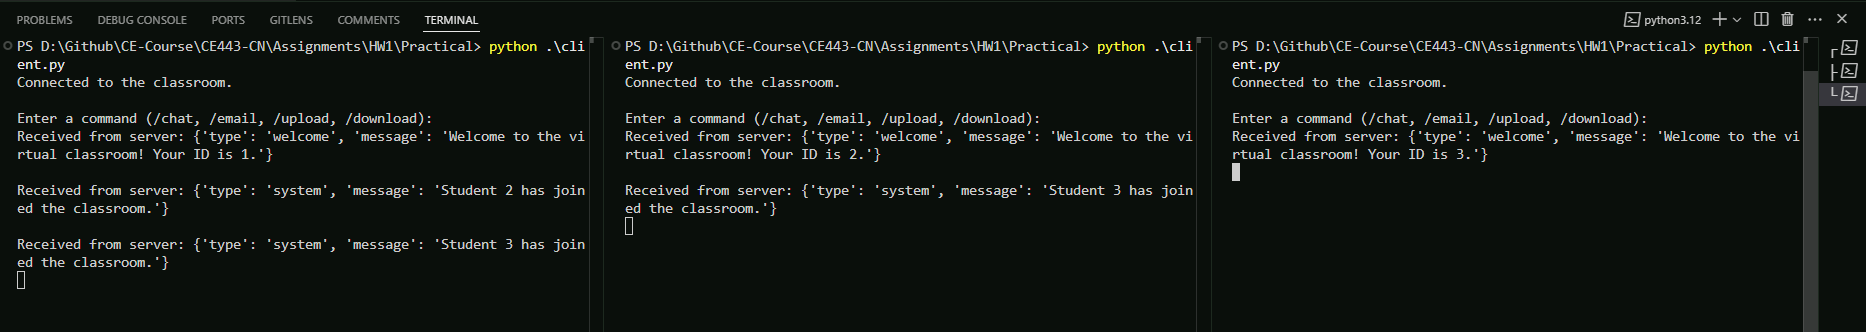
\includegraphics[width=1\linewidth]{figs/20}
		
	}
}

{
	\centering{
		
		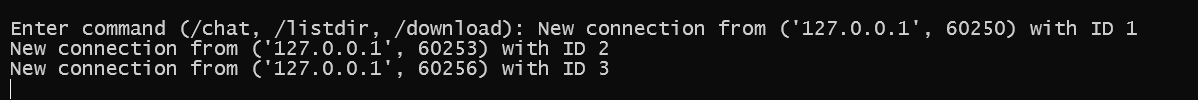
\includegraphics[width=0.65\linewidth]{figs/21}
		
	}
}

با کاربر 1 برای بقیه پیام ارسال میکنیم، میبینید که به دست استاد و باقی دانشجوها میرسد:

{
	\centering{
		
		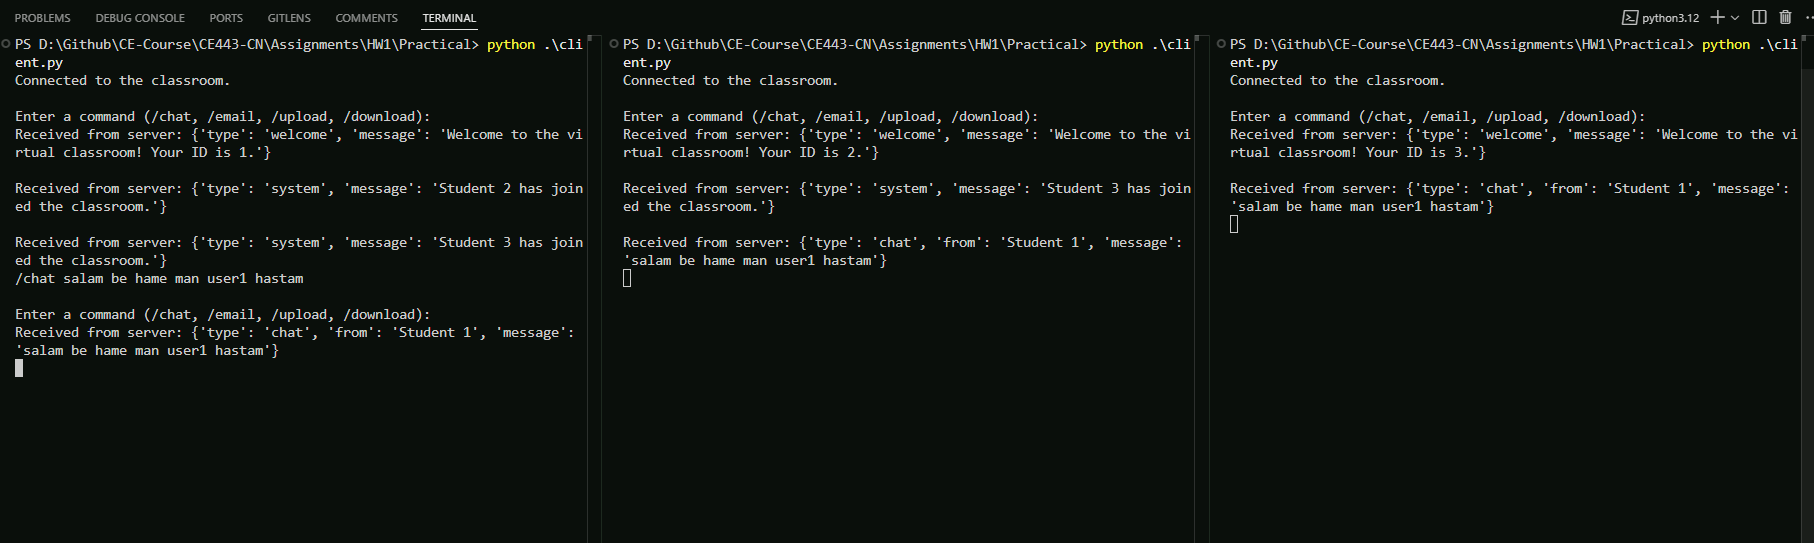
\includegraphics[width=1\linewidth]{figs/22}
		
	}
}


{
	\centering{
		
		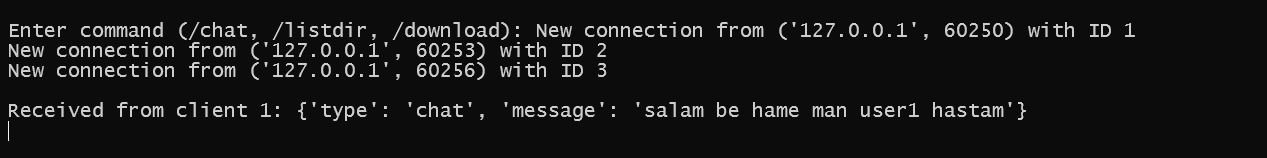
\includegraphics[width=0.65\linewidth]{figs/23}
		
	}
}

حال توسط 2 یوزر، 2 فایل مختلف را در FTP اپلود میکنیم:

{
	\centering{
		
		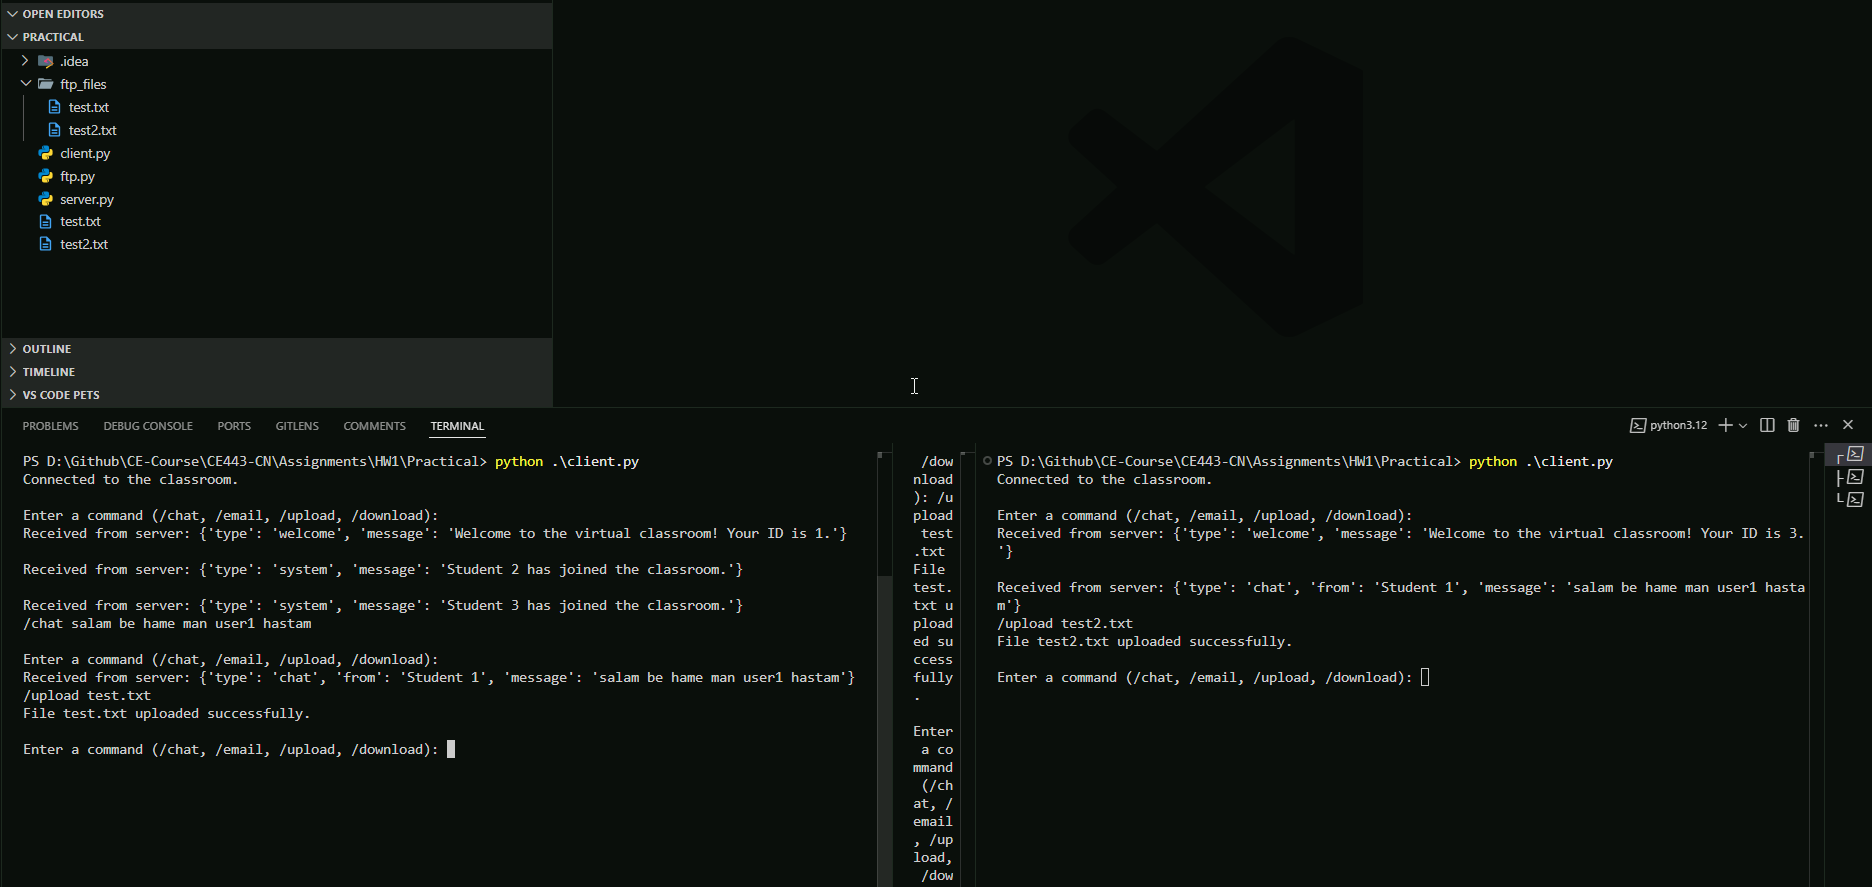
\includegraphics[width=1\linewidth]{figs/24}
		
	}
}

حال اگر درخواست دانلود بدهیم نیاز به تایید استاد است، اگر استاد تایید کند فایل 
دانلود میشود:

{
	\centering{
		
		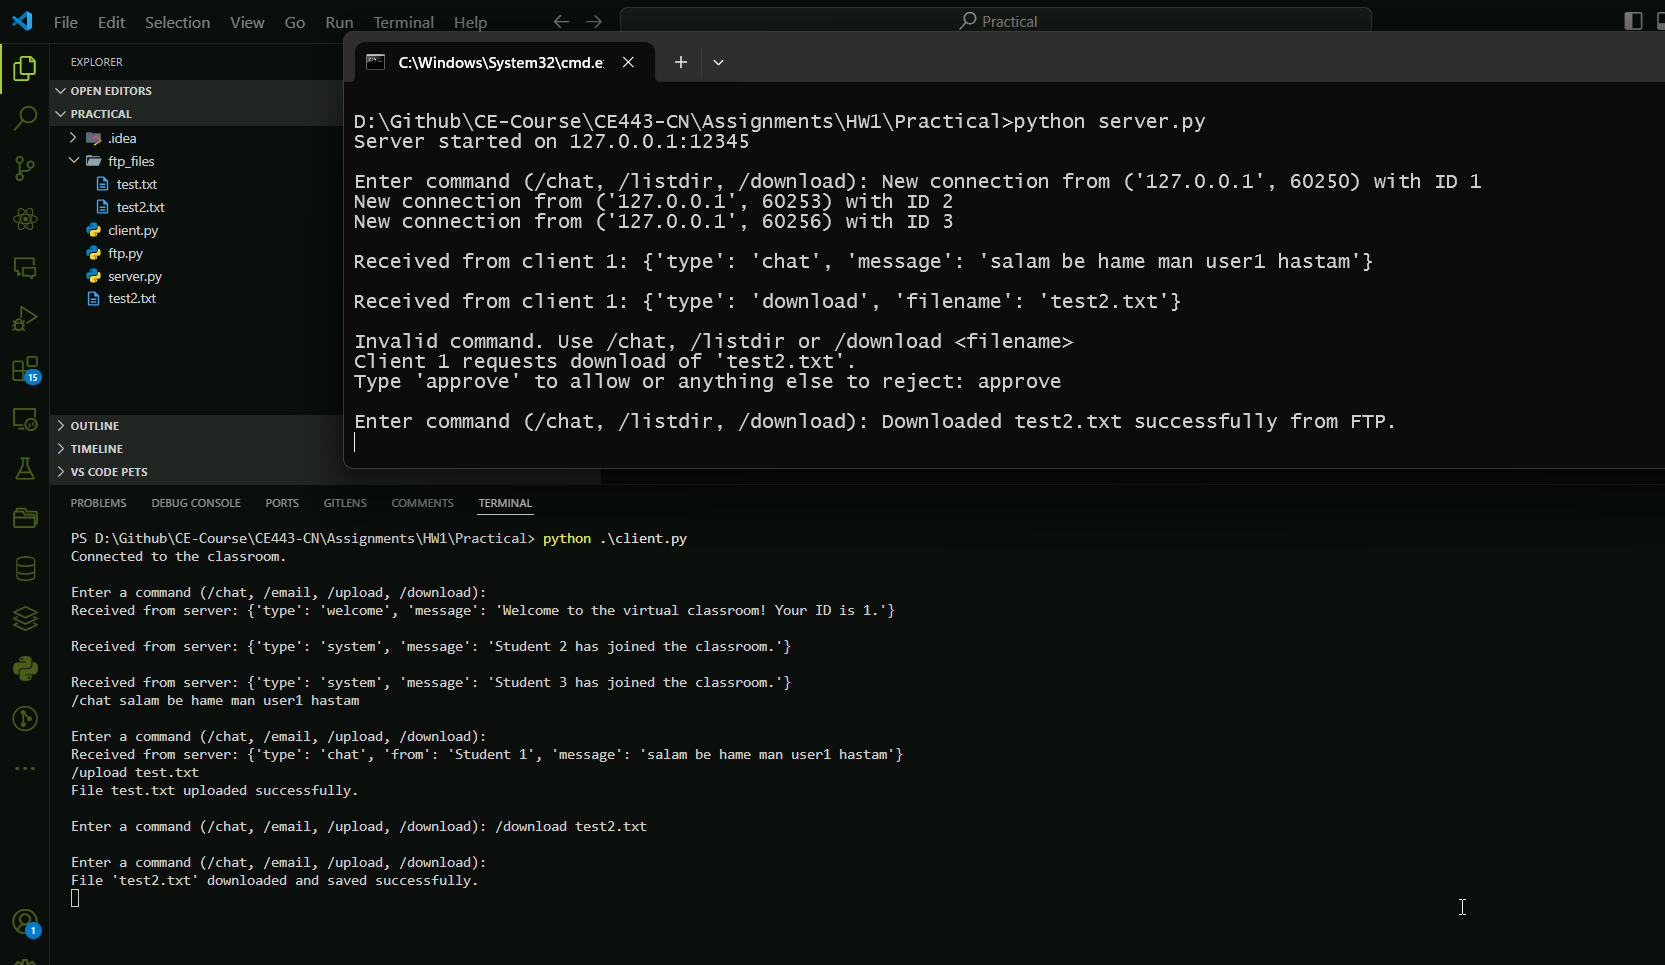
\includegraphics[width=1\linewidth]{figs/25}
		
	}
}

میبنید که کاربر درخواست دانلود میدهد و به سرور پیغام داده میشود، اگر استاد تایید کند فایل برای کاربر دانلود شده و کنار client.py ذخیره میشود. البته لاگ های اپلود فایل ها هم در کد سرور موجود است.


داخل کنسول سرور اگر بخواهیم لیست تمامی فایل ها را ببینیم:

{
	\centering{
		
		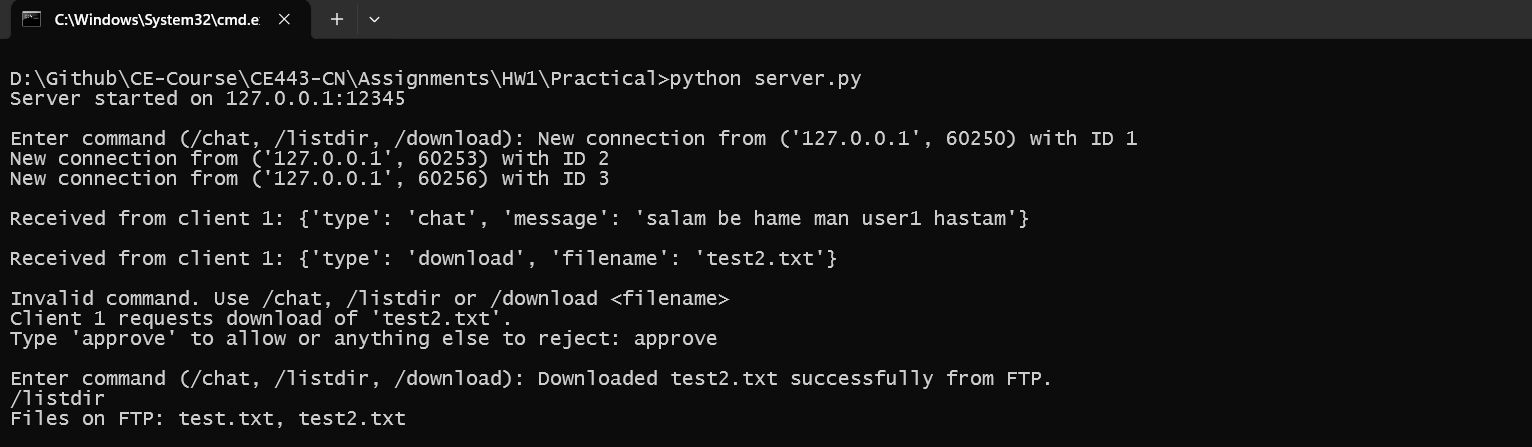
\includegraphics[width=1\linewidth]{figs/26}
		
	}
}


همچنین اگر بخواهیم از طرف استاد به بقیه پیام broadcast کنیم، به این صورت انجام میشود:

{
	\centering{
		
		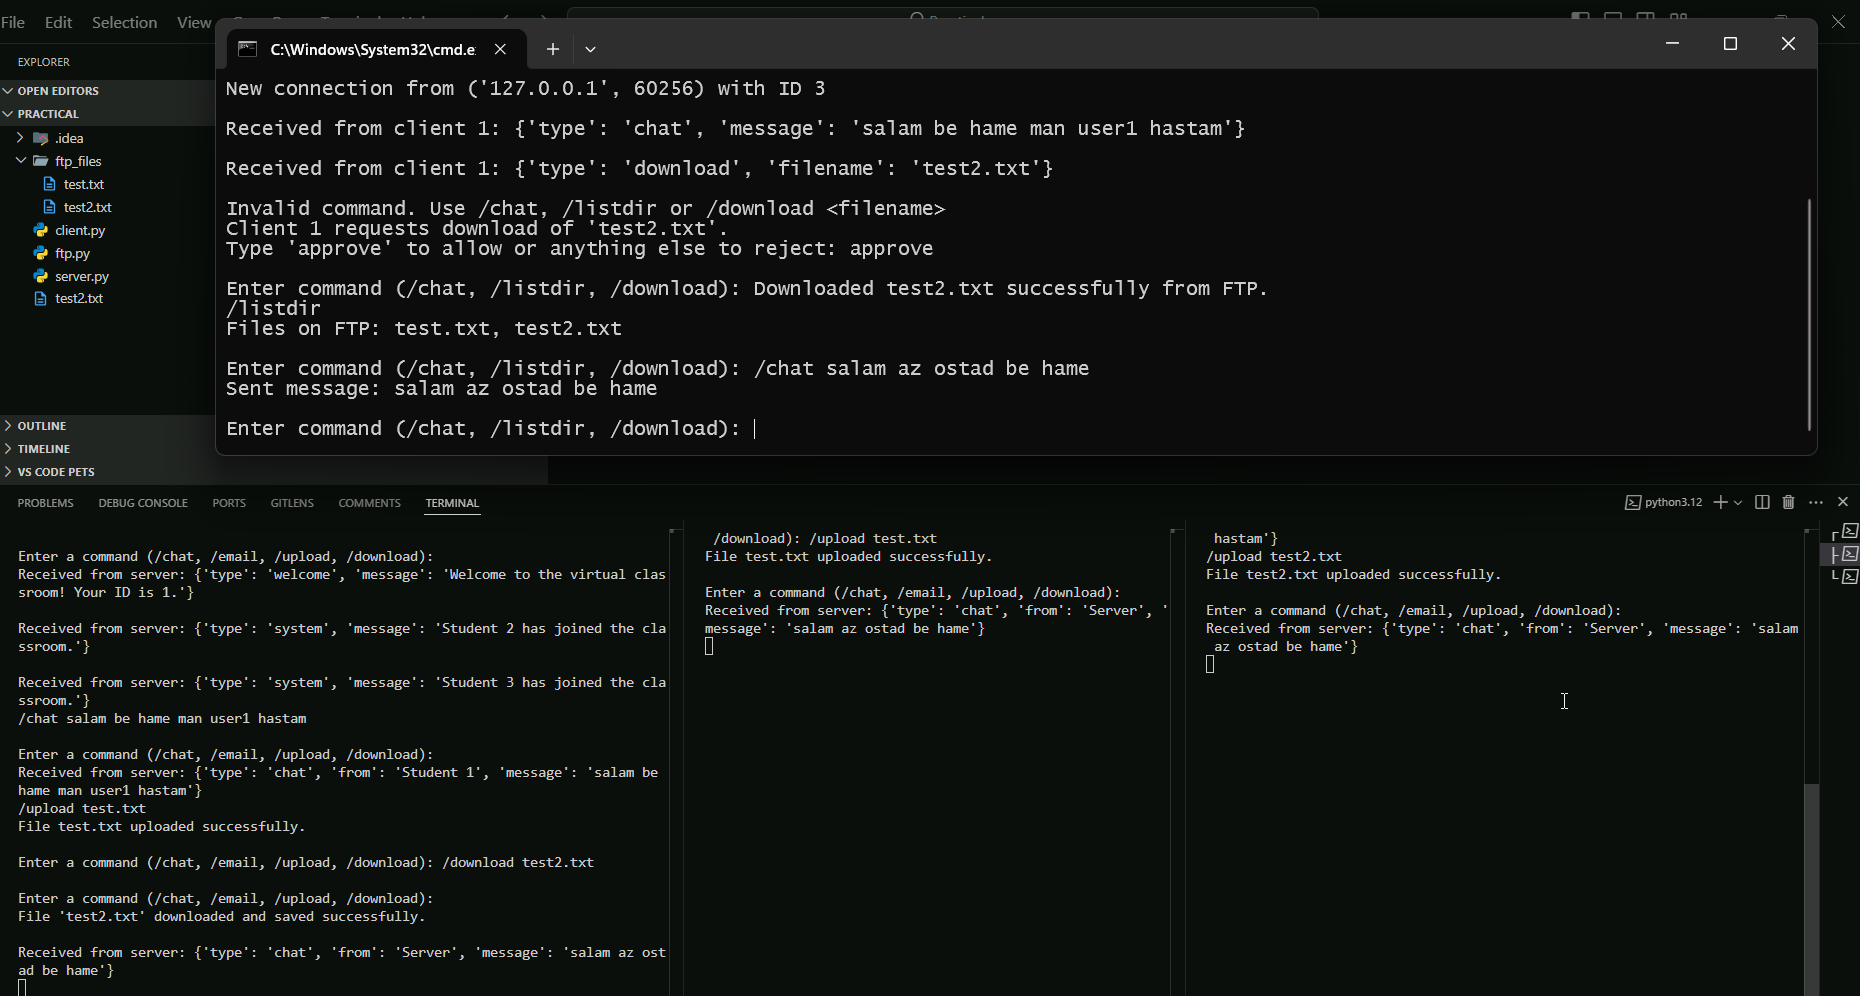
\includegraphics[width=0.8\linewidth]{figs/27}
		
	}
}


\pagebreak


همچنین استاد بدون نیاز به تایید میتواند فایل های موجود در FTP را به راحتی دانلود کند:


{
	\centering{
		
		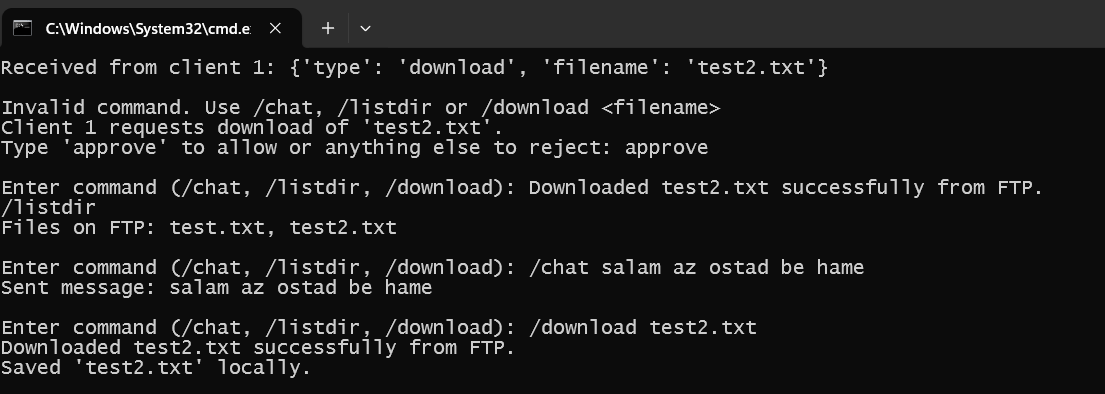
\includegraphics[width=0.6\linewidth]{figs/29}
		
	}
}

همچنین با وصل شدن به SMTP گوگل میتوان ایمیل ارسال کرد:

{
	\centering{
		
		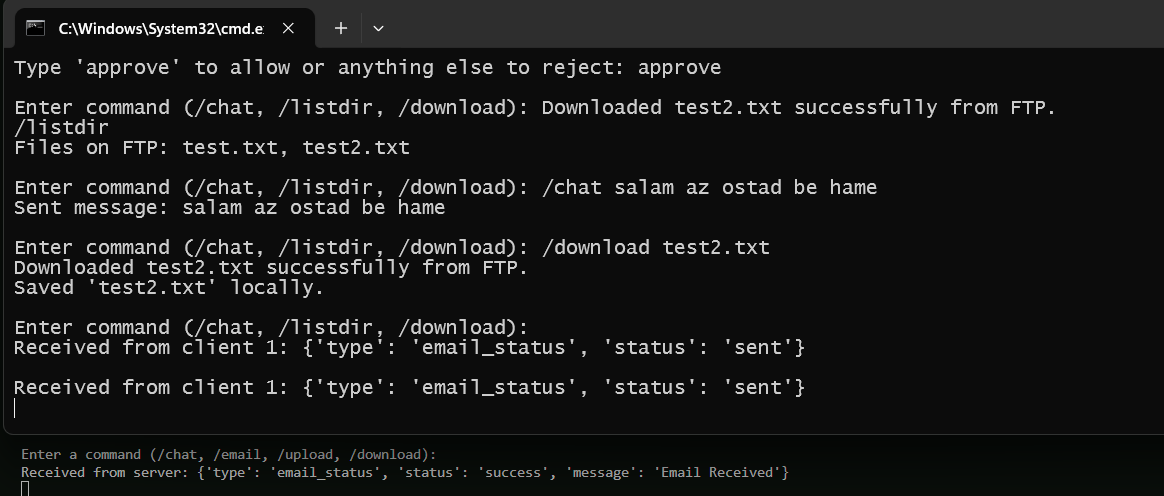
\includegraphics[width=0.6\linewidth]{figs/30}
		
	}
}


البته باید مراقب باشیم که ایمیل های ما حالت Spam نباشند. در این صورت Google اکانت ما را بن خواهد کرد. (  تجربه :)  )




